\documentclass[a4paper,12pt]{article}
\usepackage[english]{varioref}
\usepackage{setspace}
\usepackage[margin=2.54cm]{geometry}
\usepackage{pdfpages}
\usepackage[utf8]{inputenc}
\usepackage[english]{babel}
\usepackage{graphicx,subcaption}
\usepackage{graphics}
\usepackage{lscape}
\usepackage{pdflscape}
\usepackage{float}
\usepackage{textcomp}
\usepackage{amsmath}
\usepackage{hyperref}
\usepackage{fancyvrb}
\usepackage{parskip}
\usepackage{changepage}
\usepackage{enumitem}
\usepackage{tcolorbox}
\usepackage[all]{hypcap}
\usepackage{xcolor}
\usepackage{listings}
\definecolor{green}{HTML}{228B22}
\definecolor{orange}{HTML}{FFC107}
\usepackage{color}
\definecolor{dkgreen}{rgb}{0,0.6,0}
\definecolor{gray}{rgb}{0.5,0.5,0.5}
\definecolor{mauve}{rgb}{0.58,0,0.82}
\lstset{escapeinside={<@}{@>}}

\hypersetup{
    colorlinks,
    citecolor=black,
    filecolor=black,
    linkcolor=black,
    urlcolor=black
}


\lstset{frame=tb,
    language=java,
    aboveskip=3mm,
    belowskip=3mm,
    showstringspaces=false,
    columns=flexible,
    basicstyle={\small\ttfamily},
    numbers=none,
    numberstyle=\tiny\color{gray},
    keywordstyle=\color{blue},
    commentstyle=\color{dkgreen},
    stringstyle=\color{mauve},
    breaklines=true,
    breakatwhitespace=true, tabsize=3
}
\title{
	\begin{center}
	\vspace{3cm}
	\includegraphics[width=11cm, height=3cm]{images/Logo-nou-eps.jpg}
	\end{center}
	\begin{center}
	\line(1,0){340}
	\end{center}		
	DISTRIBUTED COMPUTING\\
	\vspace{2mm}
	\Large Project 2: Web service\\
	\line(1,0){340}
	\vspace{2.5cm}
	}

\author{Marc Cervera Rosell - 47980320C \vspace{1cm}}


\date{December 2022\vspace{0.5cm} \\Grau en Enginyeria Informàtica}
\onehalfspacing

\begin{document}
	\begin{titlepage}
		\maketitle
		\thispagestyle{empty}
	\end{titlepage}
	\cleardoublepage
	\newpage

\tableofcontents
\listoffigures
\thispagestyle{empty}

\newpage
\section*{UML}
\addcontentsline{toc}{section}{UML}
The UML diagram that corresponds to the used data model to solve this practical case, looks as It can be seen in the following image:
\begin{figure}[H]
    \centering
    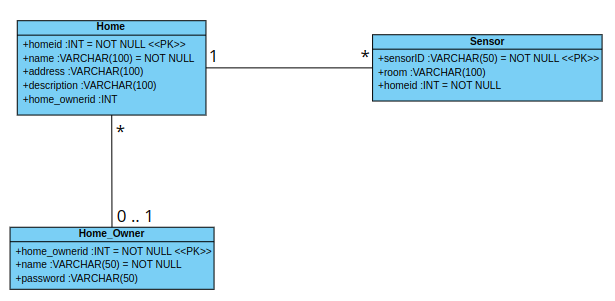
\includegraphics[scale = 0.7]{images/UML project 2.png}
    \caption{UML digram of the database}
    \label{fig:uml}
\end{figure}

\section*{Endpoints, operations, resulting codes and representations}
\addcontentsline{toc}{section}{Endpoints, operations, resulting codes and representations}
\subsection*{Endpoint /home}
\addcontentsline{toc}{subsection}{Endpoint /home}
This endpoint, has a total of four operations: POST, PUT, DELETE and GET.
\subsubsection*{POST operation}
\addcontentsline{toc}{subsubsection}{POST operation}
This operation will, firstly, get the data from the body petition and will validate it according to the \textit{home\_schema} schema. If the validation goes wrong, will raise a 400 error and an information message.\\
In case the data validation goes well, the second step of this operation will be, to check if the body petition contains a \textit{home\_ownerid}. In case, the body does not have a value for this parameter, the program will assign a default value of 1. Otherwise, will get it from the message.\\
Finally, the program will insert in the database the data. If the insertion is successful, a 201 code will be raised jointly with a message. In case of unsuccessful insertion, a 500 code will be raised jointly with an error message.\\
The insertion SQL query looks like:
\begin{lstlisting}
    INSERT INTO Home (name, address, description, home_ownerid) VALUES ('name', 'address', 'description', 'home_ownerid')
\end{lstlisting}
\subsubsection*{PUT operation}
\addcontentsline{toc}{subsubsection}{PUT operation}
As in the above operation, the first step is to get the information from the petition body and validate it. If the validation is unsuccessful, a 400 code will be raised jointly with an error message.\\
In case of a successful validation, the next step will be to check the parameters of the petition body. First of all, the program will check if the body petition contains an update for the \textit{name} field. If it contains it, will update the SQL query and if there's anything more to update, a comma will be added to the SQL query. This procedure, will be repeated for all the schema parameters.\\
The last step, will be to check if there's actually something to update in the database. If there's actually parameters to update, the program will perform the \textit{UPDATE} SQL operation. If the update is successful, a 200 code will be raised jointly with a message. Otherwise, a 500 code will be raised jointly with an error message.
Finally, if after all the checks, there's nothing to update, a 400 code will be raised jointly with a message.
\pagenumbering{arabic}
\subsubsection*{DELETE operation}
\addcontentsline{toc}{subsubsection}{DELETE operation}
This is the penultimate operation of this endpoint.\\
As is usual, the first step is to get the information to delete. Once this data is obtained, the SQL \textit{DELETE FROM} operation will be performed with the obtained data. If the SQL operation is successful, a 200 code will be raised jointly with a message. Otherwise, a 500 code will be raised.\\
The SQL query looks like:
\begin{lstlisting}
    DELETE FROM Home WHERE homeid = 'specified_homeid' and home_ownerid = specified_home_ownerid
\end{lstlisting}
\subsubsection*{GET operation}
\addcontentsline{toc}{subsubsection}{GET operation}
This is the last operation of this endpoint.\\
To perform this operation, there are two possibilities. If there's nothing specified, all the houses will be listed.
Otherwise, that is, a criteria search and a criteria value are specified, the SQL query will be conformed with this data. And the house that meets the parameters will be listed.\\
In case there isn't any house that meets the parameters, or there's not any house in the database, a 500 error will be raised jointly with an error message. Otherwise, a 200 code will be raised jointly with the result of the query.
The SQL query to list all the houses looks like:
\begin{lstlisting}
    SELECT * FROM Home
\end{lstlisting}
And the SQL query to list a specified home looks like:
\begin{lstlisting}
    SELECT * FROM Home WHERE criteria_search = criteria_value
\end{lstlisting}
\subsection*{Endpoint /home/prts/ \textless criteria \textgreater / \textless value \textgreater}
\addcontentsline{toc}{subsection}{Endpoint /home/prts/ \textless criteria \textgreater / \textless value \textgreater}
This endpoint, only has one GET operation. This operation performs the partial search.\\
The operation will list all the data of a house that meets a criteria search and a pattern of the value that is associated with the criteria search.
\begin{lstlisting}
    SELECT * FROM Home WHERE criteria_search LIKE %pattern%
\end{lstlisting}
If, for any reason, the query is unsuccessful, a 500 code will be raised jointly with an error code. Otherwise, a 200 code will be raised jointly with the result of the query.
\subsection*{Endpoint /sensor}
\addcontentsline{toc}{subsection}{Endpoint /sensor}
This endpoint has a total of two operations. These operations are: POST, DELETE.
\subsubsection*{POST operation}
\addcontentsline{toc}{subsubsection}{POST operation}
This operation's mission is to introduce new values in the database.\\
The first step is to get the data from the body and validate it according to the \textit{sensor\_schema} schema. If the validation is unsuccessful, a 400 code will be raised jointly with an error message.\\
If the validation becomes successful, the next step is to generate and execute the SQL query with the body data.\\
If the sensor creation query finishes successfully, a 201 code will be raised jointly with a message. Otherwise, a 500 code will be raised jointly with an error message.
\begin{lstlisting}
    INSERT INTO Sensor (sensorID, room, homeid) VALUES ('sensorID', 'room', 'homeid')
\end{lstlisting}
\subsubsection*{DELETE operation}
\addcontentsline{toc}{subsubsection}{DELETE operation}
This operation, works exactly in the same way as the DELETE operation of the \textit{/home} endpoint. The only difference is located in the SQL query. The \textit{/home} SQL DELETE query looks like:
\begin{lstlisting}
    DELETE FROM Home WHERE homeid = specified_homeid and home_ownerid = specified_home_ownerid
\end{lstlisting}
And the DELETE operation of this endpoint looks like:
\begin{lstlisting}
    DELETE FROM Sensor s INNER JOIN Home h ON s.homeid = h.homeid WHERE s.criteria_search = specified_criteria_search and h.home_ownerid = specified_home_ownerid
\end{lstlisting}
The fact of performing the INNER JOIN operation between the table Home and the table Sensor is to make sure that a user can only delete his own sensors.\\
If the query execution finishes successfully, a 200 code will be raised jointly with a message. Otherwise, a 500 code will be raised jointly with an error message.\\
The justification of using INNER JOIN instead of another JOIN type, is because if in one table does not exist the \textit{homeid}, the JOIN operation will not work.
\subsection*{Endpoint /home/ \textless homeid \textgreater /sensor}
\addcontentsline{toc}{subsection}{Endpoint /home/ \textless homeid \textgreater /sensor}
This endpoint, only has a GET method that allows us to list the sensor of a home.\\
This endpoint lists all the sensors of a concrete home. So, the \textit{homeid} must be provided.\\
If the query finishes successfully, a 200 code will be raised jointly with the information. Otherwise, a 500 code will be raised jointly with an error message.
The SQL query looks like:
\begin{lstlisting}
    SELECT * FROM Sensor WHERE homeid = specified_homeid
\end{lstlisting}
\subsection*{Endpoint /homeowner}
\addcontentsline{toc}{subsection}{Endpoint /homeowner}
This endpoint has a total of two operations. These operations are: GET and POST.
\subsubsection*{GET operation}
\addcontentsline{toc}{subsubsection}{GET operation}
The first step is to get the information from the body petition and validate it according to \textit{homeowner\_schema} schema. IF the validation is unsuccessful, a 400 code will be raised jointly with an error message.\\
Finally, this method will introduce in a SQL query the name of a homeowner and will return all the data related with him/her. If the query finishes successfully, a 200 code will be raised jointly with the result of the query.\\
The SQL query looks like:
\begin{lstlisting}
    SELECT * FROM Home_Owner WHERE name = 'specified_name'
\end{lstlisting}
\subsubsection*{POST operation}
\addcontentsline{toc}{subsubsection}{POST operation}
This second, and last, operation of this endpoint, will firstly get the data from the body petition and will validate it according to the \textit{homeowner\_schema} schema. IF the validation is unsuccessful, a 400 code will be raised jointly with an error message.\\
So, in this case the SQL query will look like:
\begin{lstlisting}
    INSERT INTO Home_Owner (name, password) VALUES (name_value, password_value)
\end{lstlisting}
If the insertion is successful, a 201 code will be riased jointly with a message. Otherwise, a 500 code will be raised jointly with an error message.
\subsection*{Endpoint /homeowner/check/ \textless home\_ownerid \textgreater}
\addcontentsline{toc}{subsection}{Endpoint /homeowner/check/ \textless home\_ownerid \textgreater}
This endpoint, only has a GET operation. This operation will list all the information about a homeowner that has the specified ID.\\
Hence, the SQL query will look like:
\begin{lstlisting}
    SELECT * FROM Home_Owner WHERE home_ownerid = specified_home_ownerid
\end{lstlisting}
If the ID of the specified homeowner cannot be found in the database, a 404 code will be raised jointly with an error message. Otherwise, a 200 code will be raised jointly with a message.\\
If, for any reason, the query is “unable” to get the data (database connection), a 500 code will be raised jointly with an error message.
\subsection*{Endpoint /homeowner/ \textless home\_ownerID \textgreater /homes}
\addcontentsline{toc}{subsection}{Endpoint /homeowner/ \textless home\_ownerID \textgreater /homes}
This endpoint only has a GET operation that will list all the homes from a homeowner.\\
So, the SQL query will look like:
\begin{lstlisting}
    SELECT * FROM Home WHERE home_ownerid = specified_home_ownerid
\end{lstlisting}
As is usual, if the query finishes successfully, a 200 code will be raised, jointly with the result of the wuery and if, for any reason, the query fails, a 500 code will be raised jointly with an error message.
\subsection*{Endpoint /alldata}
\addcontentsline{toc}{subsection}{Endpoint /alldata}
This endpoint, has a GET operation and a POST operation.
\subsubsection*{GET operation}
\addcontentsline{toc}{subsubsection}{GET operation}
This operation, lists all the homes from a homeowner.\\
In order to do it, the program will try to execute the following SQL query:
\begin{lstlisting}
    SELECT * FROM Home_Owner ho left join Home h on ho.home_ownerid = h.home_ownerid left join Sensor s on h.homeid = s.homeid
\end{lstlisting}
If the query is successful, a 200 code is raised jointly with the result of the query. Otherwise, a 500 code is raised jointly with an error code.
The justification of using the LEFT JOIN operation it's because in case a house does not have any sensors or a user does not have any houses, at least we can still get its user information.
\subsubsection*{POST operation}
\addcontentsline{toc}{subsubsection}{POST operation}
The first step, is to get the information from the body petition.\\
In this part, each insertion will have its own query. It's to say, there's going to be a query for the \textit{Home\_Owner} table insertion, another for the \textit{Home} table insertion and another one for the \textit{Sensor} table insertion.\\
In case there's nothing to insert into one of these tables, the SQL query will not be executed, due to each SQL query is inside an \textit{if} statement that checks into which table we want to insert.\\
If all the queries, that have to be executed, finis successfully, a 200 code is raised jointly with a message. Otherwise, a 400 code is raised jointly with an error message.
\subsection*{Endpoint /sensor/ \textless sensorID \textgreater}
\addcontentsline{toc}{subsection}{Endpoint /sensor/ 
\textless sensorID \textgreater}
This endpoint, only has a GET method.\\
This endpoint will connect to the MongoDB of the first project and will get the temperatures of the specified sensor.
\newpage
\section*{Some project justifications}
\addcontentsline{toc}{section}{Some project justifications}
In this report's section are going to be justified the design decisions.
\subsection*{Why Flask?}
\addcontentsline{toc}{subsection}{Why Flask?}
Flask is a web framework, it’s a Python module that lets programmers develop web applications easily.
So, why is Flask a good choice? In addition, to all the Python advantages, Flask some advantages more.\\
The Flasks design is lightweight and modular. Therefore, it's easy to transform it into a web application or framework when one needs very few extensions without weighing much.\\
Flask is ORM-agnostic.\\
The basic foundation of API is very nicely shaped and made coherent.\\
The documentation of Flask is very comprehensive, filled with lots and well-structured examples. Users can even try out some sample applications to really get the real feel of Flask.\\
Flask can handle HTTP requests easily with the help of its functionalities.\\
It's highly flexible. Its configuration is even more flexile than that of Django, which gives its users plenty of solutions for every product they need.
\subsection*{Why MySQL?}
\addcontentsline{toc}{subsection}{Why MySQL?}
MySQL is globally for being the most secure and reliable database management system used in popular web applications like WordPressm Drupal, Joomla, Facebook, and Twitter.\\
MySQL offers unmatched scalability to facilitate the management of deeply embedded apps using a smaller footprint, even in massive warehouses that stack terabytes of data. On-demand flexibility is the star feature of MySQL.\\
MySQL features a distinct storage-engine framework that facilitates system administrators to configure the MySQL database server for a flawless performance. MySQL is designed to meet even the most demanding applications while ensuring optimum speed, full-text indexes and unique memory caches for enhanced performance.\\
MySQL comes with the assurance of 24X7 uptime and offers a wide range of high availability solutions like specialized cluster servers and master/slave replication configurations.\\
MySQL tops the list of robust transactional database engines available on the market. With features like complete atomic, consistent, isolated, durable transaction support, multi-version transaction support, and unrestricted row-level locking, it is the go-to solution for full data integrity. It guarantees instant deadlock identification through server-enforced referential integrity.\\
With the average download and installation time being less than 30 minutes, MySQL means usability from day one. Whether your platform is, MySQL is a comprehensive solution with self-management features that automate everything from space expansion and configuration to data design and database administration.
\subsection*{Why Swagger?}
\addcontentsline{toc}{subsection}{Why Swagger?}
Swagger provides a unique and convenient platform to document, test, and write API structures.\\
Swagger provides a method to automate the documentation, which means Swagger picks up the methods with GET, PUT, POST, DELETE attributes and prepares the documentation by itself. Further, if any changes are implemented, then the Swagger documentation is automatically updated.\\
Swagger provides a UI integrated page where all the API methods are listed and enables the user to test any method that is required from the UI.\\
Swagger does the documentation in a conventional way (OpenAPI) which means it is in a machine-readable language. If a user starts the documentation first, Swagger will write the structure of the API automatically based on the written documentation. The API logic relies on the developer and business requirements, but the structure will be written by Swagger itself.\\
The user does not need separate applications to test APIs. Just configure Swagger once in the project and access it through a URL to test the APIs.\\
Swagger provides immense support for a wide range of platforms, languages, and domains.
\section*{Execution cases}
\addcontentsline{toc}{section}{Execution cases}
In order to demonstrate the correct functioning of the API, I'm going to use the \textit{Stoplight Studio} application, and I'm going to follow the steps of the \textit{WS demo} section of the statement.\\
Before starting with the demos, it must be said that the IDs will not start in “normal” indexes because of previous tests.
\newpage
\subsection*{WS demo's first step}
\addcontentsline{toc}{subsection}{WS demo's first step}
This first step requires creating three different houses, with the two first ones with a similar description.
\begin{figure}[H]
    \centering
    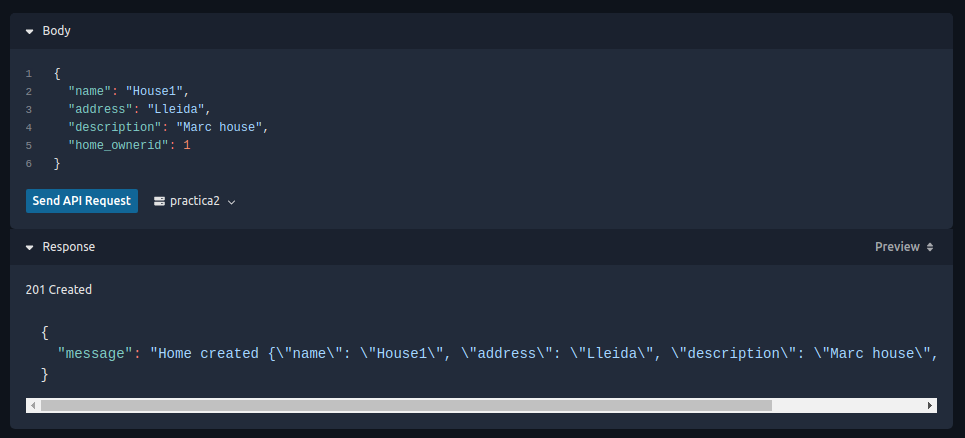
\includegraphics[scale = 0.5]{images/House 1 creation.png}
    \caption{Creation of the first house}
    \label{fig:house1C}
\end{figure}
\begin{figure}[H]
    \centering
    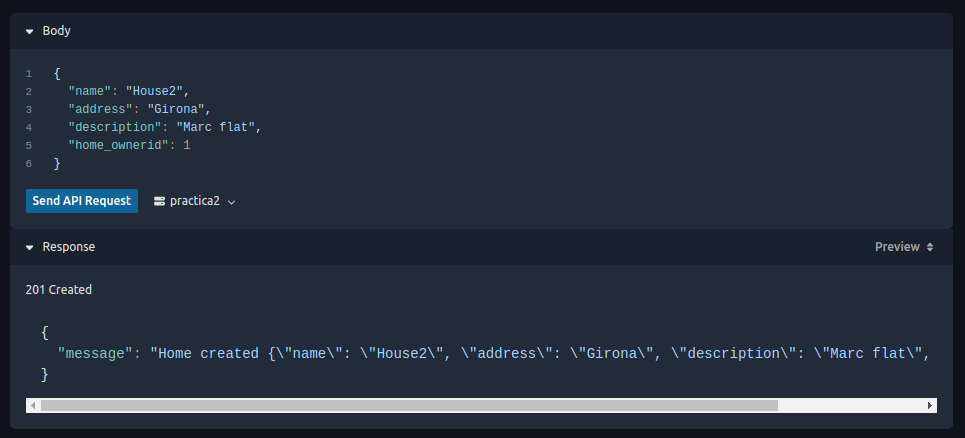
\includegraphics[scale = 0.5]{images/House 2 creation.png}
    \caption{Creation of the second house}
    \label{fig:house2C}
\end{figure}
\begin{figure}[H]
    \centering
    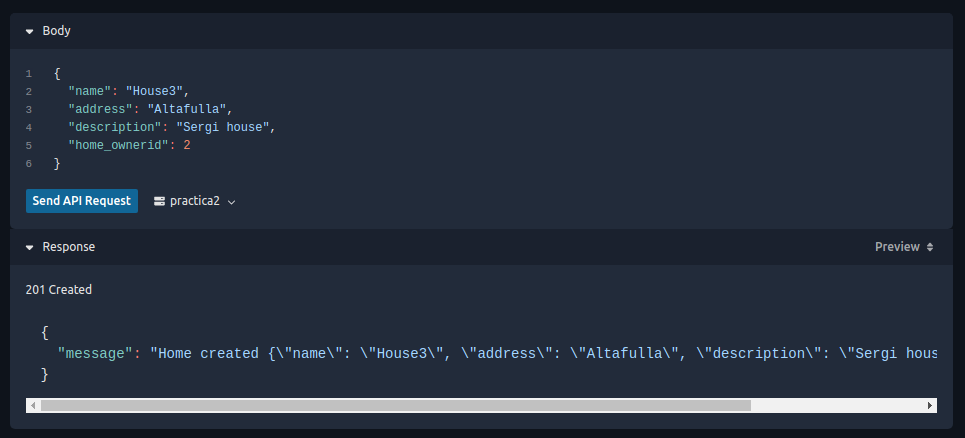
\includegraphics[scale = 0.5]{images/House 3 creation.png}
    \caption{Creation of the third house}
    \label{fig:house3C}
\end{figure}
As it can be seen, every request has become successful due to a 201 has been raised jointly with the information that has been introduced.
\subsection*{WS demo's second step}
\addcontentsline{toc}{subsection}{WS demo's second step}
This step, requires modifying the description of the third house.
\begin{figure}[H]
    \centering
    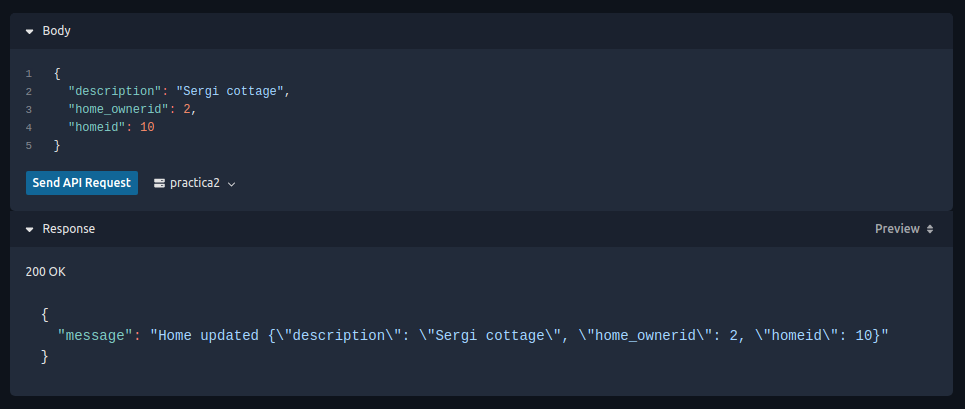
\includegraphics[scale = 0.5]{images/House 3 update.png}
    \caption{Update of the third house}
    \label{fig:house3U}
\end{figure}
As it can be seen, the third's house description update, is successful because a 200 code is raised.
\subsection*{WS demo's third step}
\addcontentsline{toc}{subsection}{WS demo's third step}
This step requires searching a home by its description.
\begin{figure}[H]
    \centering
    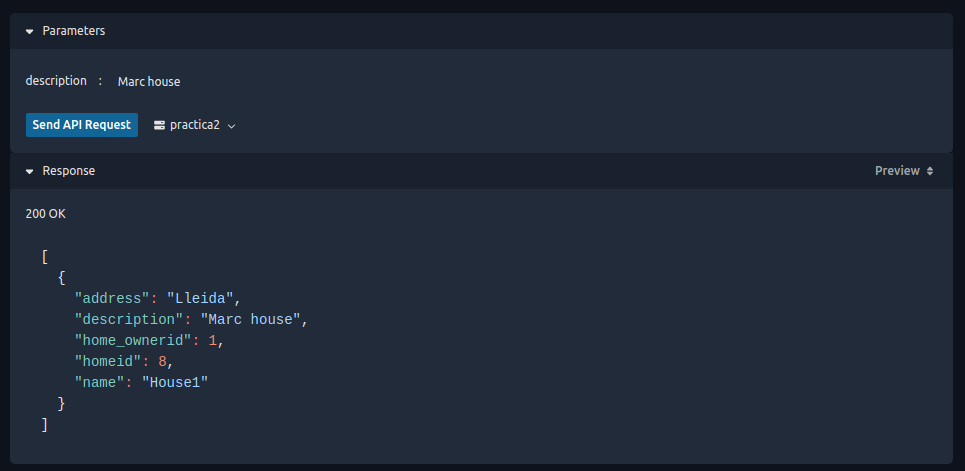
\includegraphics[scale = 0.5]{images/Full search.png}
    \caption{Full search}
    \label{fig:full}
\end{figure}
As it can be seen, the operation finishes successfully, due to a 200 code is raised.
\newpage
\subsection*{WS demo's fourth step}
\addcontentsline{toc}{subsection}{WS demo's fourth step}
This fourth step requires deleting the second home.
\begin{figure}[H]
    \centering
    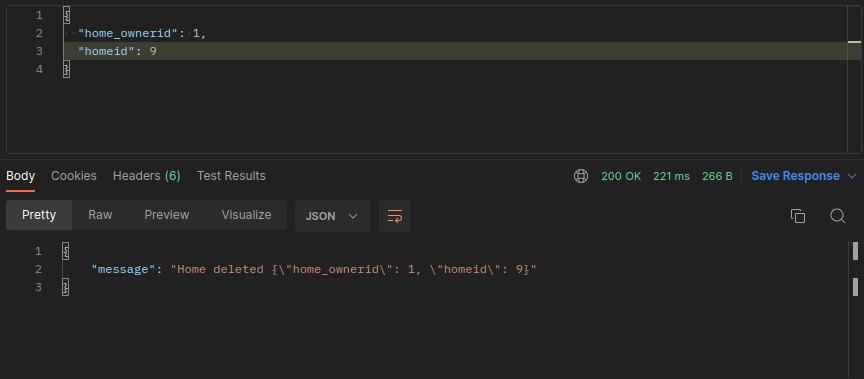
\includegraphics[scale = 0.5]{images/House 2 deletion.png}
    \caption{House 2 deletion}
    \label{fig:house2D}
\end{figure}
As it can be seen, the DELETE operation performs normally due to a 200 code is raised jointly with an informative message.\\
This operation has been performed with Postman because, in \textit{Stoplight studio}, for some reason does not work.
\begin{figure}[H]
    \centering
    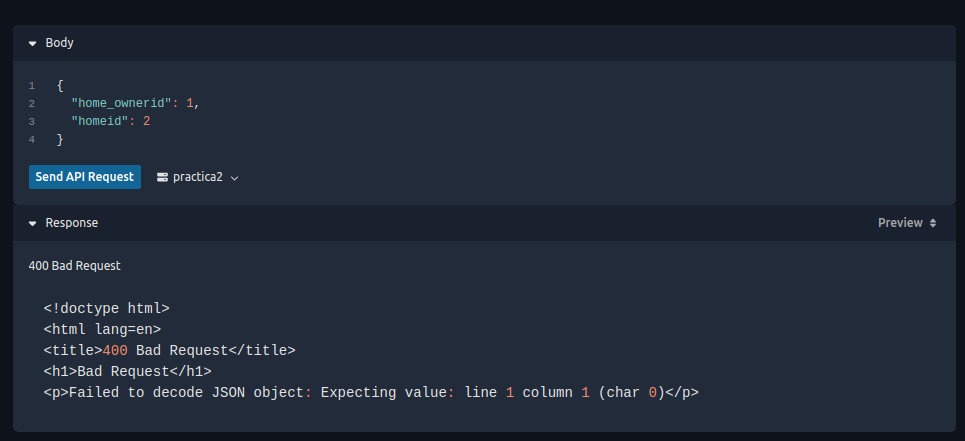
\includegraphics[scale = 0.5]{images/Stopligh studio 400 error.png}
    \caption{Stoplight studio error while performing the DELETE operation}
    \label{fig:stoplight}
\end{figure}
It seems that, for some reason, does not get the data.
\subsection*{WS demo's fifth step}
\addcontentsline{toc}{subsection}{WS demo's fifth step}
This section of the demo demands to list all the houses
\begin{figure}[H]
    \centering
    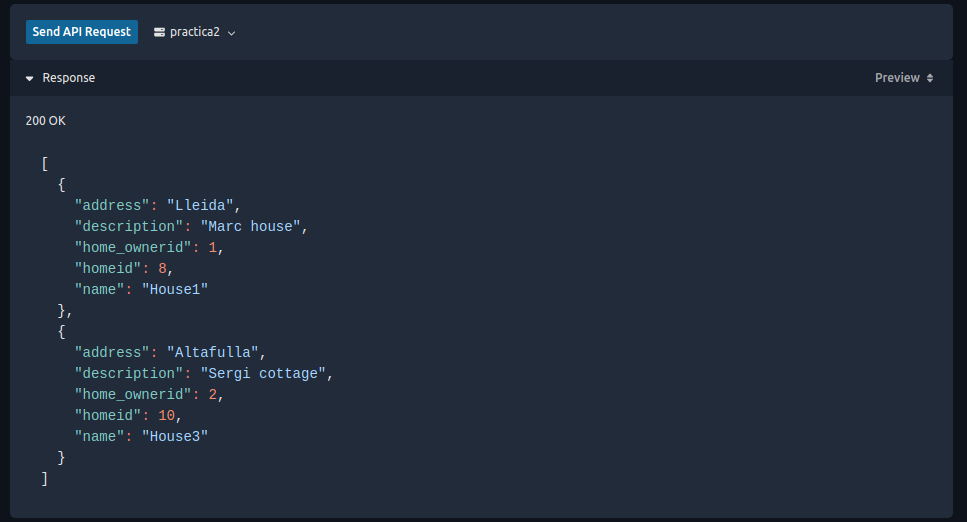
\includegraphics[scale = 0.5]{images/List all houses.png}
    \caption{All houses in the system}
    \label{fig:allhouses}
\end{figure}
As it can be seen, the operation finishes successfully, due to a 200 code is raised.
\subsection*{WS demo's sixth step}
\addcontentsline{toc}{subsection}{WS demo's sixth step}
This part of the demo, requires creating two sensors for the first home.
\begin{figure}[H]
    \centering
    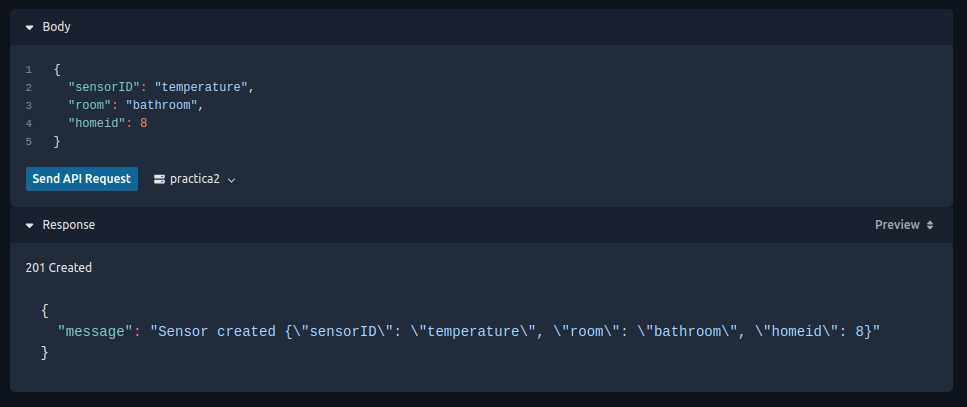
\includegraphics[scale = 0.5]{images/Sensor 1 created.png}
    \caption{Sensor 1 creation}
    \label{fig:sensor1C}
\end{figure}
\begin{figure}[H]
    \centering
    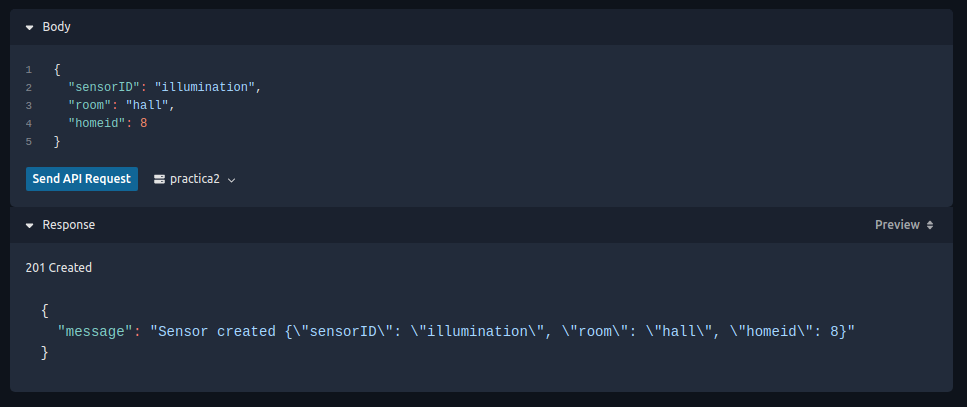
\includegraphics[scale = 0.5]{images/Sensor 2 created.png}
    \caption{Sensor 1 creation}
    \label{fig:sensor1C}
\end{figure}
As it can be seen, the creation of both sensors finish successfully due to a 201 code is raised.
\subsection*{WS demo's seventh step}
\addcontentsline{toc}{subsection}{WS demo's seventh step}
In this part, the statement requires listing all the sensors in the first home. In this case, list all the sensors will coincide with the sensors that have just been created.
\begin{figure}[H]
    \centering
    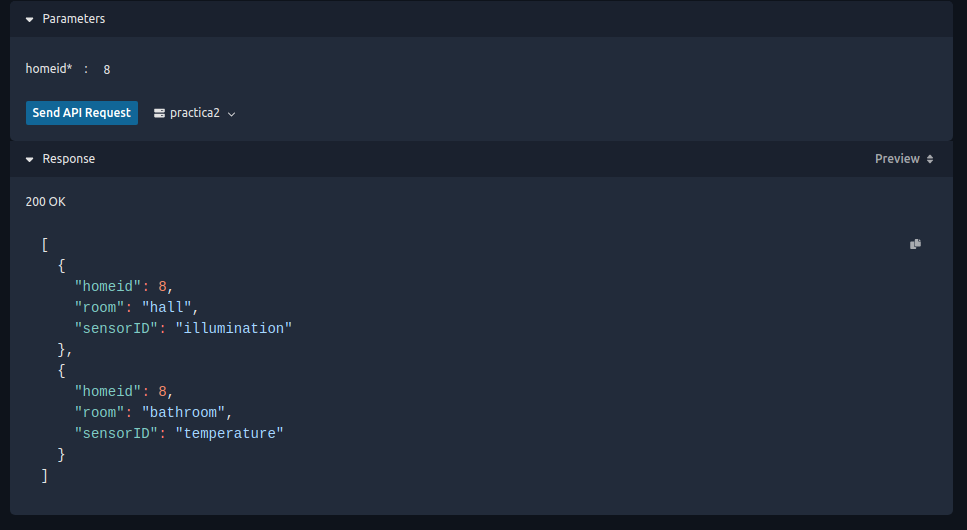
\includegraphics[scale = 0.5]{images/First house sensors.png}
    \caption{Sensors in the first house}
    \label{fig:sensorshouse1}
\end{figure}
As it can be seen, the GET operations work well due to a 200 code is raised.
\subsection*{WS demo's eighth step}
\addcontentsline{toc}{subsection}{WS demo's eighth step}
This section demands creating two different users.
\begin{figure}[H]
    \centering
    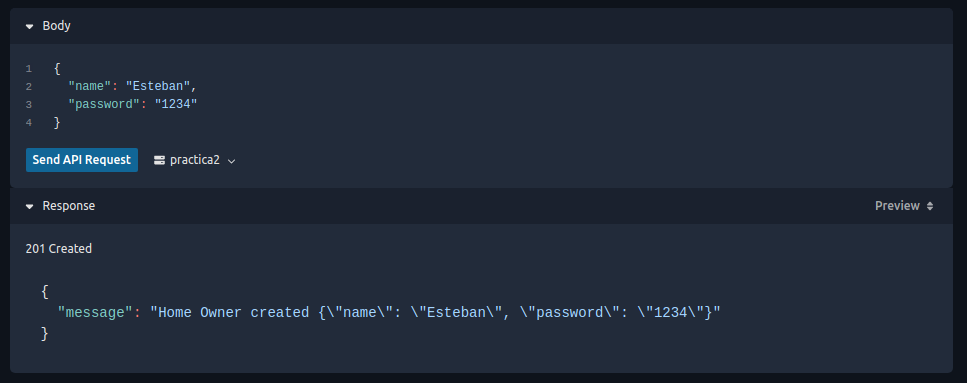
\includegraphics[scale = 0.5]{images/User 1 created.png}
    \caption{User 1 creation}
    \label{fig:user1C}
\end{figure}
\begin{figure}[H]
    \centering
    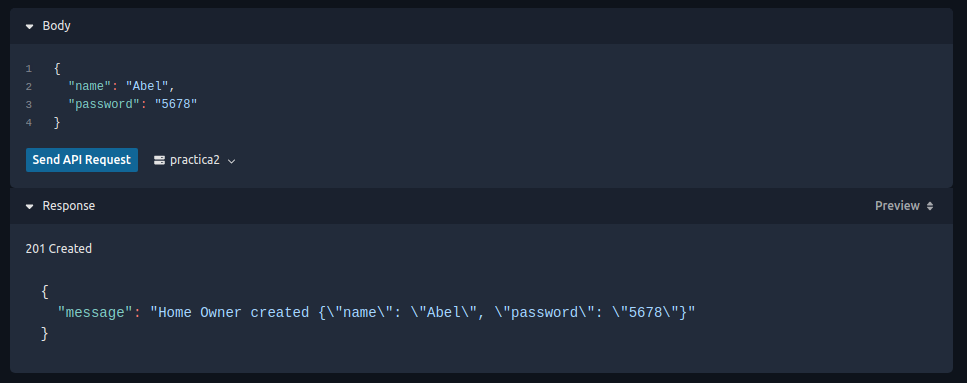
\includegraphics[scale = 0.5]{images/User 2 created.png}
    \caption{User 2 creation}
    \label{fig:user2C}
\end{figure}
As it can be seen, the users are created successfully due to a 201 code is raised.
\subsection*{WS demo's ninth step}
\addcontentsline{toc}{subsection}{WS demo's ninth step}
In this part, we've to assign a new house to each new user.\\
If we take a look in the \textit{Home\_Owner} table, we will see that the user \textit{Esteban} has an ID of 4 and the user \textit{Abel} has an ID of 5. So, when creating the houses, the field \textit{home\_ownerid} will have a value of 4 or 5.
\begin{figure}[H]
    \centering
    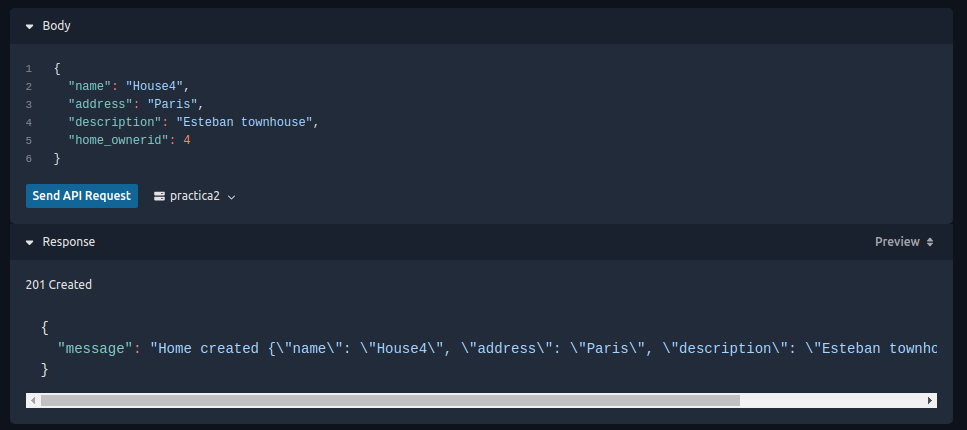
\includegraphics[scale = 0.5]{images/Esteban house.png}
    \caption{Esteban's house creation}
    \label{fig:esteban}
\end{figure}
\begin{figure}[H]
    \centering
    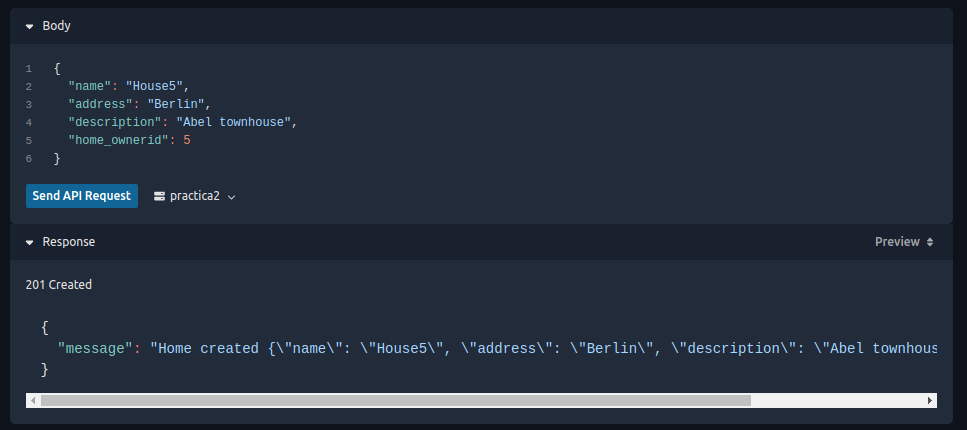
\includegraphics[scale = 0.5]{images/Abel house.png}
    \caption{Abel's house creation}
    \label{fig:abel}
\end{figure}
The operation finishes successfully due to a 201 code is raised.
\subsection*{WS demo's tenth step}
\addcontentsline{toc}{subsection}{WS demo's tenth step}
Now, the house of the second created user (Abel) has to be deleted.
\begin{figure}[H]
    \centering
    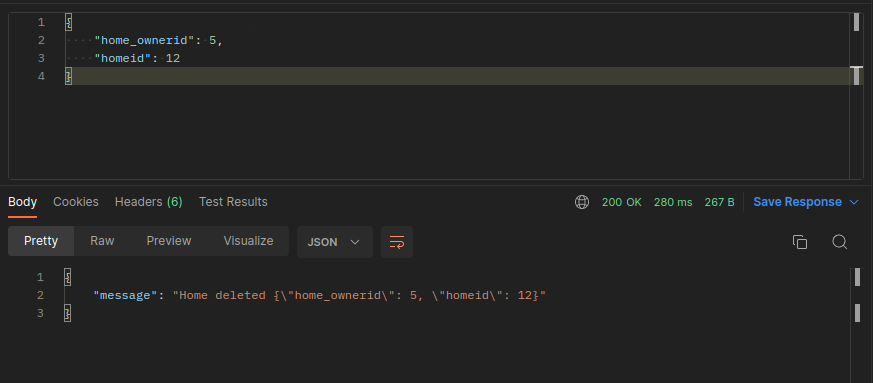
\includegraphics[scale = 0.5]{images/Abel house deleted.png}
    \caption{Abel's house deletion}
    \label{fig:abelD}
\end{figure}
As it can be seen, the operation is performed in Postman for the same reason as the last DELETE operation, and as it can be seen too, the deletion finishes successfully due to a 200 code is raised.
\subsection*{WS demo's eleventh step}
\addcontentsline{toc}{subsection}{WS demo's eleventh step}
Now, a house has to be searched (by its description) another time, but this time, the description is not going to be provided fully.
\begin{figure}[H]
    \centering
    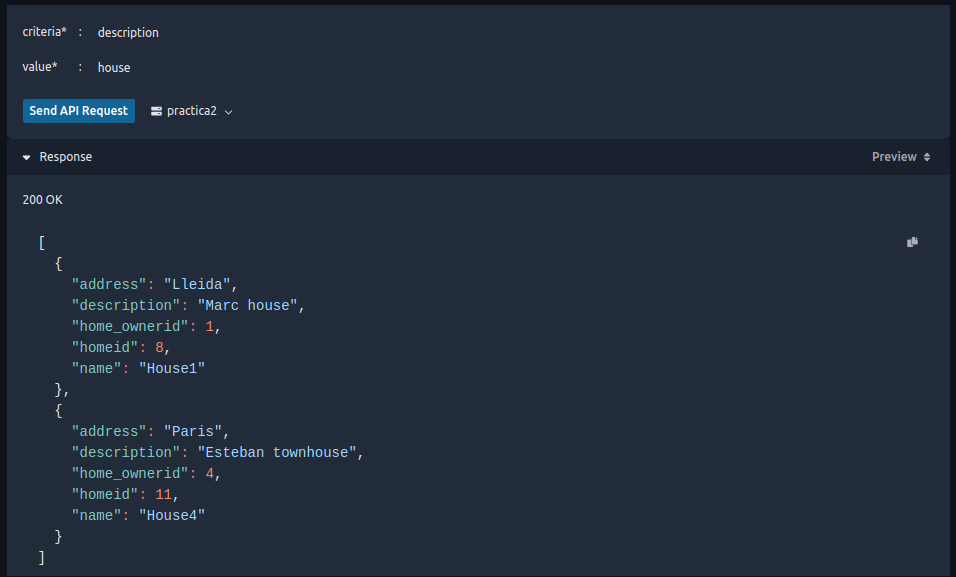
\includegraphics[scale = 0.5]{images/Partial search.png}
    \caption{Partial search}
    \label{fig:partial}
\end{figure}
As it can be seen, a house can be searched by part of its description. This can be affirmed due to a 200 code is raised.
\subsection*{WS demo's twelfth step}
\addcontentsline{toc}{subsection}{WS demo's twelfth step}
Due to there're two users as the result of the partial search, only the user \textit{Esteban} and its information will be shown.
\begin{figure}[H]
    \centering
    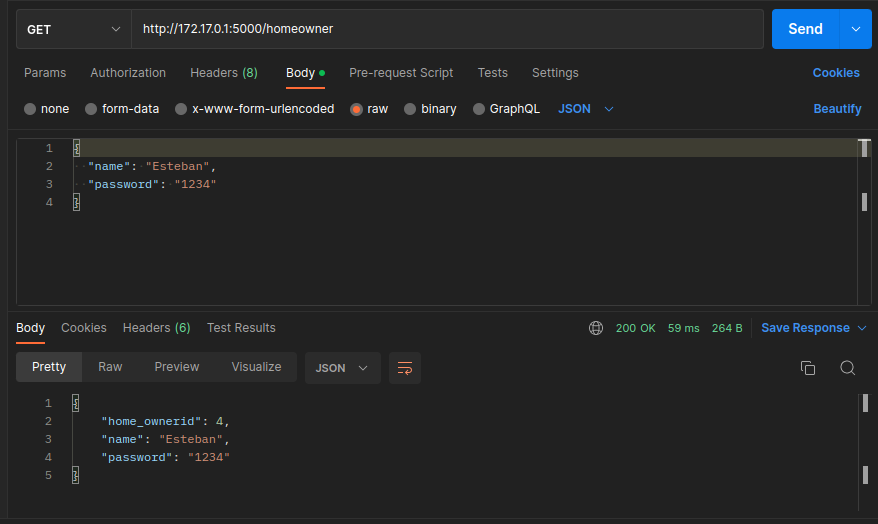
\includegraphics[scale = 0.5]{images/Esteban GET.png}
    \caption{Esteban's information}
    \label{fig:estebanG}
\end{figure}
As it can be seen, the operation finishes successfully due to a 200 code is raised.
\subsection*{WS demo's thirteenth step}
\addcontentsline{toc}{subsection}{WS demo's thirteenth step}

\subsection*{WS demo's fourteenth step}
\addcontentsline{toc}{subsection}{WS demo's fourteenth step}
In this penultimate part, an ID of an existing user must be checked.
\begin{figure}[H]
    \centering
    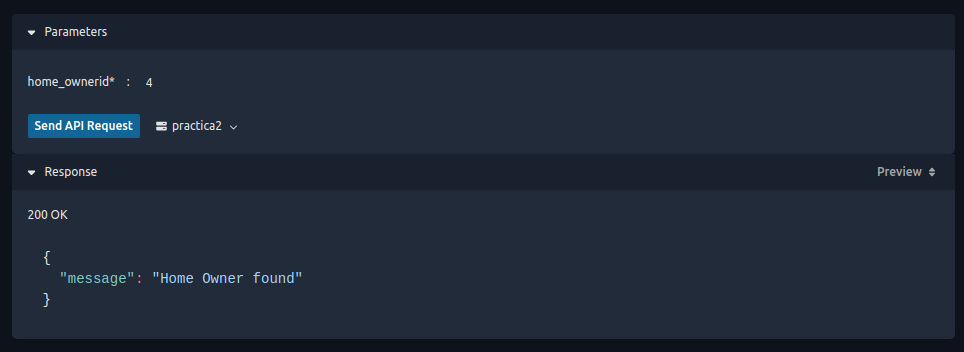
\includegraphics[scale = 0.5]{images/check id existent.png}
    \caption{Result of checking an ID of an existing user}
    \label{fig:idExist}
\end{figure}
As it can be seen, a 200 code is raised jointly with an informative message that allows the users to know that the ID is present in the database.
\subsection*{WS demo's fifteenth step}
\addcontentsline{toc}{subsection}{WS demo's fifteenth step}
Finally, a non-existing ID must be checked.
\begin{figure}[H]
    \centering
    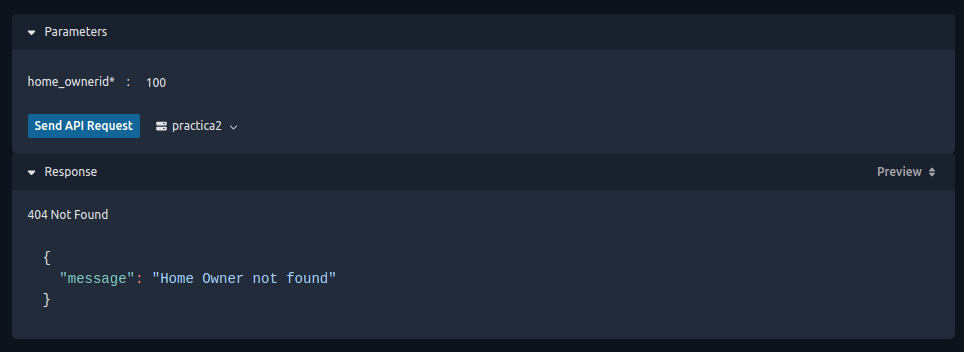
\includegraphics[scale = 0.5]{images/check id non existing.png}
    \caption{Result of checking a non-existing ID}
    \label{fig:idNoExist}
\end{figure}
As it can be seen, a 404 code is raised jointly with an error message informing that the user ID does not exist.
\newpage
\section*{Source code}
\addcontentsline{toc}{section}{Source code}
The code of the project can be found in a \textit{.zip} file in the virtual campus' assignment, and can be found too in the following GitHub link: \href{https://github.com/marc7666/Distributed-computing-course.git}{\underline{GitHub repository}}. In order to see the whole project, you must be sure you're in the “main” branch and then, enter into the \textit{Projects} folder and, finally, in the \textit{Project 2} folder.
\section*{Hours dedicated to the project}
\addcontentsline{toc}{section}{Hours dedicated to the project}
The total hours dedicated to the project are:
\begin{itemize}
    \item Programming part: More or less 50 hours.
    \item Testing part: More or less 20 hours.
    \item Documentation part: More or less 15 hours.
\end{itemize}



\end{document}
